\documentclass[conference, 11pt]{IEEEtran}
\usepackage{xcolor}
\usepackage{cite}
\usepackage{url}
\usepackage{graphicx}
\usepackage{enumitem}
\usepackage{parskip}
\usepackage{booktabs}
\usepackage{graphicx}
\usepackage[font=small,labelfont=bf]{caption}
\usepackage{subcaption}

\begin{document}
\newcommand{\derek}[1] {\textcolor{blue}{\textbf{[Derek: #1]}}}
\newcommand{\mina}[1] {\textcolor{green}{\textbf{[Mina: #1]}}}
\newcommand{\mazyar}[1] {\textcolor{orange}{\textbf{[Mazyar: #1]}}}
\newlist{questions}{enumerate}{2}
\setlist[questions,1]{label=RQ\arabic*.,ref=RQ\arabic*}
\setlist[questions,2]{label=(\alph*),ref=\thequestionsi(\alph*)}

\title{Phylogenetic and Structural Analysis of BC200 and Hominoidea Homologs}

\author{Derek Robinson, Mina Emadi, Mazyar Ghezelji\\
University of Victoria\\
Victoria, Canada \\
\{drobinson, minaemadi, mazyarghezelji\}@uvic.ca}

\maketitle

\begin{abstract}
  TODO 
\end{abstract}

\section{Introduction}\label{sec:intro}

Alzheimer's disease (AD) is a neurodegenerative disease which greatly affects the lives of those who are diagnosed and those who care for the diagnosed. 
In the United States, 6.2 million patients are estimated to be living with AD and it is the sixth leading cause of death for American adults \cite{AlzheimersDisease}. 
In Canada, over 747,000 patients are living with AD, or another form of dementia \cite{ADcanada}. 
Symptoms of AD range from memory loss and poor judgement in mild cases to the inability to communicate and seizures in severe cases \cite{alzheimersSigns}.

AD involves multiple cell types and signaling pathways \cite{zhang2021role}, as such, the collective knowledge of AD is spread across many different domains. 
This spread of knowledge means that fully understanding AD in humans is difficult, let alone understanding the disease in other species of the hominoidea superfamily.
Finch and Austad argue that with our current understanding of AD, it is not possible to determine if AD is uniquely human \cite{finch2015commentary}. 
As such, this paper explores one facet of AD pathogenesis, the long non-coding RNA (lncRNA) BC200. 
BC200 has been implicated in AD as it upregulates the expression of b-site APP-cleaving enzyme1 (BACE1) \cite{li2018identification,zhang2021role}. 
The upregulation of BACE1 in turn leads to higher levels of beta-amyloid (A$\beta$) in the brain, thus, disrupting cell function \cite{li2018identification,zhang2021role}. 

In hopes of better understanding how AD may affect other species in the hominoidea superfamily, specifically, the role that hominoidea homologs of BC200 play in AD, we answer the following research questions:

\begin{questions}
  \item What does the phylogenetic tree of BC200 look like?
  \item What structural differences exist between BC200 and its four most closely related hominoidea homologs?
\end{questions}

The following paper is structured as follows: section \ref{sec:background} gives background into BC200 and the role it plays in AD, section \ref{sec:methods} lays out the methods used for selecting BC200 homologs and performing both the phylogenetic structural analysis, section \ref{sec:results} presents the results of our analysis, section \ref{sec:discussion} discusses the relevancy of the results, and section \ref{sec:conclusion} concludes the paper.

\section{Background}\label{sec:background}

\subsection{What is BC200?}

Brain Cytoplasmic 200 lncRNA (BC200) is a 200 nucleotide long RNA transcript which is found mostly in the brain \cite{tiedge1993primary}. 
As a non-coding RNA, BC200 is not translated into protein but can be used as a potential therapeutic target and biomarker due to its regulatory role in biological processes involved in disease development \cite{zhang2021role,mus2007dendritic}. 
This lncRNA has recently been studied extensively because of its role in regulating translation and inhibiting its initiation, as well as its impacts in the pathogenesis of Alzheimer's disease and cancer \cite{zhang2021role,tiedge1993primary}. 
Because of the crucial role of BC200 in translation control, it impacts the synthesis of dendritic proteins which facilitates long-term plastic changes at the synapse \cite{mus2007dendritic}.

\subsection{The Relation Between AD and BC200}

Alzheimer's disease (AD) is a neurodegenerative disease resulting from synaptic plasticity failure in neurons \cite{mus2007dendritic}. 
It is a complex disease, meaning that it involves multiple cell types and signaling pathways \cite{zhang2021role}.

AD is thought to occur due to the accumulation of two proteins in the brain. 
One of them is beta-amyloid (A$\beta$) which accumulates in neurons, forms plaques, and disrupts cell functions. 
The other one is hyper-phosphorylated tau protein which in abnormal levels can form neurofibrillary tangles in neurons and block synaptic transmissions \cite{zhang2021role}.

A$\beta$, a cleavage product of the amyloid precursor protein (APP), is generated by b-site APP-cleaving enzyme1 (BACE1) and $\gamma$-secretase complex, and it strongly influences the pathogenesis of AD. 
Inhibition of BACE1 activity and the subsequent reduction in A$\beta$ levels may cure or prevent AD\cite{li2018identification,zhang2021role}.

BC200 facilitates AD pathogenesis by upregulating A$\beta$ production through the modulation of BACE1 expression. 
The inhibition of BC200 significantly suppresses BACE1 expression, increases cell viability and reduces cell apoptosis in an AD model, and these effects are reversed by BC200 over-expression \cite{li2018identification,zhang2021role}.

Many researches have demonstrated the important role of BC200 in AD. 
El Mus \emph{et al.} show that there are steady decline in BC200 level from age 49 to 86, but, in AD brain its level was substantially higher\cite{mus2007dendritic}. 
They also observe that BC200 expression is increased in brain areas that are involved in AD and it is parallel with severity of disease. 
Huanyen Li \emph{et al.} establish an AD cell model over expressing A$\beta$1-42 to observe the effects of BC200 on the cell viability and apoptosis and to investigate the associated underlying mechanisms\cite{li2018identification} . 
They observe that BC200 and BACE1 were increased upon treatment with A$\beta$1-42, and inhibition of BC200 rescued this A$\beta$1-42-mediated dysfunction, as indicated by the interaction of BC200 directly targeting BACE1. 
Moreover, inhibition of BC200 increased AD cell growth and reduced cells apoptosis. 
They demonstrate that BC200 is a potent positive regulator of BACE1 in AD cells and in conclusion, lncRNA BC200 facilitates AD pathogenesis by up-regulating A$\beta$ through BACE1.  					 			 		 	 

\section{Materials and Methods}\label{sec:methods}

\subsection{Selection of lncRNAs}\label{sec:lncRNA-selection}
The lncRNA BC200 was selected for phylogenetic and structural analysis due to the role it plays in AD as discussed in section \ref{sec:background}. 
The homologs of BC200 were selected as a result of an NCBI Blast \cite{blastTool} search. 
Specifically, Megablast \cite{morgulis2008database} with default parameters was used as it is able to compare closely related sequences \cite{amirmahani2018phylogenetic}. 
From the Blast results, the top six sequences which are known BC200 homologs as indicated by the inclusion of BC200 in their name were chosen. 
Two of the top hits in the Blast results were complete bacterial artificial chromosome sequences for pan troglodytes. 
Inclusion of these two sequences (accession numbers: AC185986.3, AC183594.3) caused errors in the analysis software described in section \ref{sec:phylo} and section \ref{sec:structure}, as such we did not consider these full chromosome sequences in our analysis. 
Table \ref{tbl:accession} outlines the sequence name including the organism and the accession number of each of the chosen sequences. 

\begin{table}[ht]
  \centering
  \caption{lncRNA Sequence Information}
  \label{tbl:accession}
  \begin{tabular}{lc}
    \toprule
    Organism Name & Sequence Accession Number \\
    \midrule
    Homo sapiens    & NR\_001568.1 \\
    Pongo pygmaeus  & AF067780.1 \\
    Pan paniscus    & AF067778.1 \\
    Gorilla gorilla & AF067779.1 \\
    Macaca mulatta  & AF067784.1 \\
    Hylobates lar   & AF067781.1 \\
    Papio hamadryas & AF067782.1 \\
    \bottomrule
  \end{tabular}
\end{table}

\subsection{Phylogenetic Analysis}\label{sec:phylo}

The lncRNA sequences in table \ref{tbl:accession} were subject to phylogenetic analysis.
The phylogenetic tree was built with the MEGA11 \cite{tamura2021mega11} bioinformatics software. 
First the sequences outlined in table \ref{tbl:accession} were aligned using the MEGA11 alignment module. 
The multiple sequence alignment was performed using the MUSCLE algorithm with default parameters. 
Once the multiple sequence alignment had been performed in MEGA11, it was then possible to build the phylogenetic tree. 

The phylogenetic tree was built using the maximum likelihood statistical method and Tamura-Nei substitution model \cite{tamura1993estimation, tamura2004prospects}. 
The bootstrap method was used as a test of phylogeny with 500 replications.
In order to further support the phylogenetic tree, estimates of evolutionary divergence were also calculated by MEGA11 \cite{tamura2021mega11}. 
Analyses were conducted using Maximum Composite Likelihood and the Tamura-Nei model \cite{tamura1993estimation, tamura2004prospects}. 
All ambiguous positions were removed for each sequence pair (pairwise deletion option). 

\subsection{Structural Analysis}\label{sec:structure}

In order to find RNA secondary structure of BC200 and three of closest homologs of it, we used FORNA, a platform for drawing the secondary RNA structure \cite{kerpedjiev2015forna}. 
FORNA is able to draw the RNA secondary structure from the dot bracket notation provided by the user or from the minimum free energy (MFE) structure as calculated by RNAFold \cite{lorenz2011viennarna}. 
As this analysis aims at computationally determining a secondary structure, the latter option of using the MFE structure was employed. 
Each of the five structures present in section \ref{sec:results-structure} was drawn individually. 
First, we analyzed BC200 structure to get a better understanding of its function in body. 
Knowing that BC200 structure consist of three main domains, we also look at its homologs from this view point. 
Comparing each homolog structure to BC200, we divided them to three main domains like BC200 structure and based on each part function we analyzed the structural differences.

\subsection{Finding Alu Domains}

Alu elements are elements of DNA that can excise and then get re-introduced into the genome. 
They called retrotransposons, also they are very common in human and primate genomes \cite{dombroski1994vivo}. 
In order to find them, we used Dfam website (https://www.dfam.org/). 
The Dfam database is an open collection of Transposable Element DNA sequence alignments, hidden Markov Models (HMMs), consensus sequences, and genome annotations. 
By using the sequence search we find the Alu domains of the BC200 and its homologs. 
Comparing the Alu domain structure gives us a suitable result for the RNA function.

\subsection{Finding Conserved Parts of BC200}
Over many generations, random mutations and deletions can change nucleic acid sequences in the genome of an evolutionary lineage. 
Chromosomal rearrangement may also recombine or delete sequences. 
Conserved sequences are sequences which persist in the genome despite such forces, and have slower rates of mutation than the background mutation rate\cite{kimura1974some}.
One of the best ways for visualize conserved sequences during evolution, is multiple sequence alignment. 
Here, we aligned BC200 and the four most related homologs with each other to find the conserved parts of the sequence. 
We used Clustal Omega for aligning the sequences \cite{madeira2019embl}. 
The CLUSTAL format includes a plain-text key to annotate conserved columns of the alignment, denoting conserved sequence (*), conservative mutations (:), semi-conservative mutations (.), and non-conservative mutations ( ). 
The output format is in ClustalW, and the guide tree is shown below.

\begin{figure}[ht]
  \centering
  \label{fig:Guide-tree}
  
\includegraphics[width=0.4\textwidth]{figs/guidetree.png}
  \caption{Multiple Sequence Alignment Guide Tree}
\end{figure}

\section{Results}\label{sec:results}

\derek{Add in a few small paragraphs tying in each section of the results to one another}

\subsection{Phylogenetic Tree of BC200}

The results of the phylogenetic analysis can be found in figure \ref{fig:phylo-tree}. 
The tree shows that the Homo sapiens BC200 lncRNA and the Gorilla gorilla BC200 lncRNA are likely to share a common ancestor. 
Similarly, the BC200 homologs from Pan paniscus and Hylobates lar are likely to share a common ancestor. 
This is also the case for the BC200 homologs from Macaca mulatta, Papio hamadryas, and Pongo pygmaeus. 

\begin{figure}[ht]
  \centering
  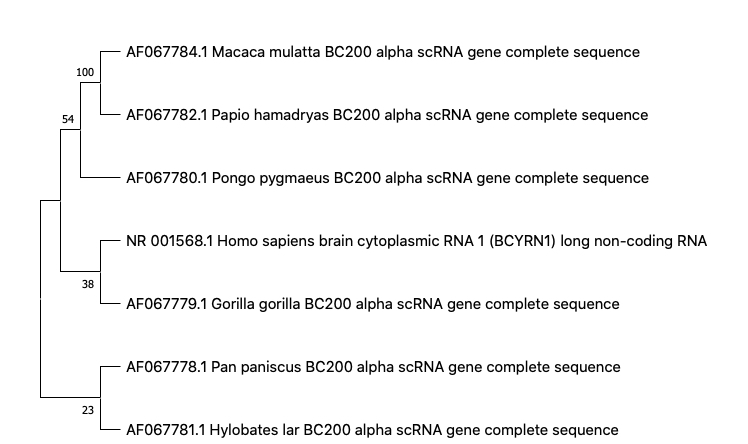
\includegraphics[width=0.485\textwidth]{figs/phylogenetic-tree.jpg}
  \caption{Phylogenetic tree of BC200 and hominoidea homologs. The numbers at each node are the bootstrap support values obtained by maximum likelihood.}
  \label{fig:phylo-tree}
\end{figure}

Additionally, table \ref{tbl:distances} shows the pairwise distances between sequences which estimate the evolutionary divergence between sequences. 
The evolutionary divergence estimates show that the four most closely related homologs of BC200 found in other hominoidea come from Pan paniscus (AF067778.1), Pongo pygmaeus (AF067780.1), Hylobates lar (AF067781.1), and Gorilla gorilla (AF067779.1). 
Thus, the aforementioned BC200 homologs (AF067778.1, AF067780.1, AF067781.1, AF067779.1) are the closest relatives of BC200 and have their secondary structure analyzed in section \ref{sec:results-structure}.

\begin{table*}[h]
  \centering
  \caption{Estimates of Evolutionary Divergence between Sequences}
  \label{tbl:distances}
  \begin{tabular}{lcccccc}
    \toprule
    Accession Number \\
    \midrule
    NR\_001568.1 \\
    AF067780.1 & 0.01023 \\
    AF067778.1 & 0.00503 & 0.02169 \\
    AF067779.1 & 0.03070 & 0.02890 & 0.01709 \\ 
    AF067784.1 & 0.03088 & 0.04573 & 0.03802 & 0.05235 \\
    AF067781.1 & 0.02561 & 0.02763 & 0.01562 & 0.02439 & 0.04353 \\ 
    AF067782.1 & 0.03120 & 0.04478 & 0.03947 & 0.04731 & 0.00852 & 0.04259 \\
    \bottomrule
  \end{tabular}
\end{table*}

\subsection{Structural difference between BC200 and its homologs}\label{sec:results-structure}

Brain cytoplasmic 200 long non-coding RNA (or BC200 lncRNA) is a 200 nucleotide RNA transcript that is found predominantly in the brain. 
Its primary function is regulating translation by inhibiting its initiation. 
It's role in AD is not fully understood, but research shows that lncRNA BC200 facilitates AD pathogenesis by upregulating AB through BACE1. 
Pathologically, AD is characterized by an imbalance in the production and clearance of amyloid-beta in the brain leading to plaque formation \cite{li2018identification}.
The BC200 structure consist of three main parts: A-rich domain, Alu domain and unique domain \cite{jung2014rna}.

\begin{figure}[h]
  \centering
  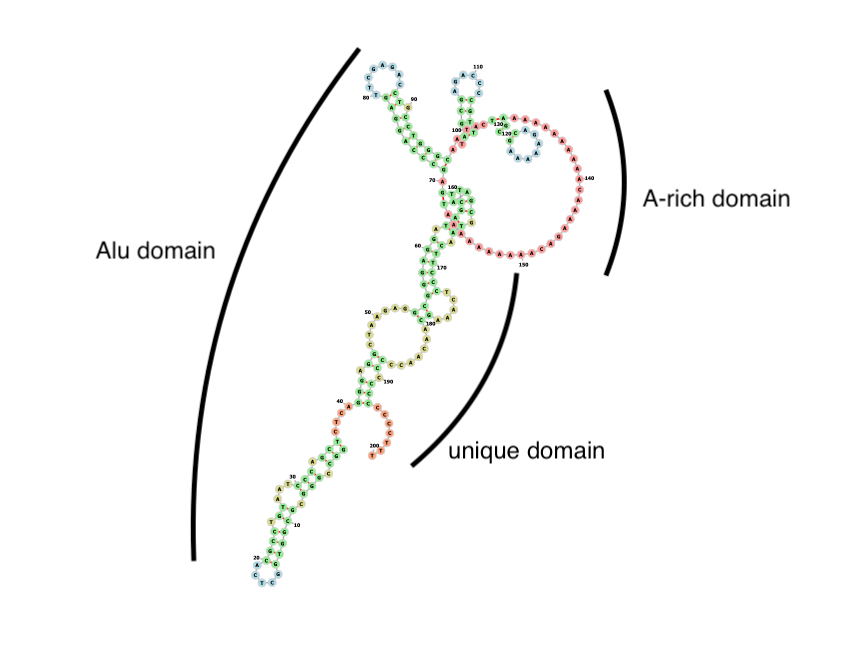
\includegraphics[width=0.4\textwidth]{figs/rna-6.png}
  \caption{BC200 RNA Secondary Structure}
  \label{fig:bc200-structure}
\end{figure}

Finding the Alu domain of BC200 and its homologs( supplementary info), we concluded that the Alu domain between human BC200 and its Select seq Pan paniscus homolog are completely the same. There are slight differences between human BC200 and its Pongo pygmaeus homolog. On the other hand the alu domain between human BC200 and its gorilla gorilla and Hylobates lar have strong differences.
The Alu domain of the mammalian signal recognition particle (SRP) comprises the heterodimer of proteins SRP9 and SRP14 bound to the 5′ and 3′ terminal sequences of SRP RNA \cite{weichenrieder2000structure}. 
So, their function in brain may be different from one another, even though there may be high similarity between their sequences. 
Figures \ref{fig:gorilla-structure}, \ref{fig:pan-structure}, and \ref{fig:pongo-structure} show the RNA secondary structure of the three most closely related BC200 homologs from great apes (hominidae). 
Additionally, we have chosen to depict the RNA secondary structure of the Hylobates lar BC200 homolog in Figure \ref{fig:hylobates-structure}. 
While Hylobates lar is not a great ape, it is still part of the hominoidea superfamily, and Phylogenetic analysis revealed that it was closely related to BC200.

\begin{figure*}[h]
  \centering
  \begin{subfigure}[b]{0.4\textwidth}
    \centering
    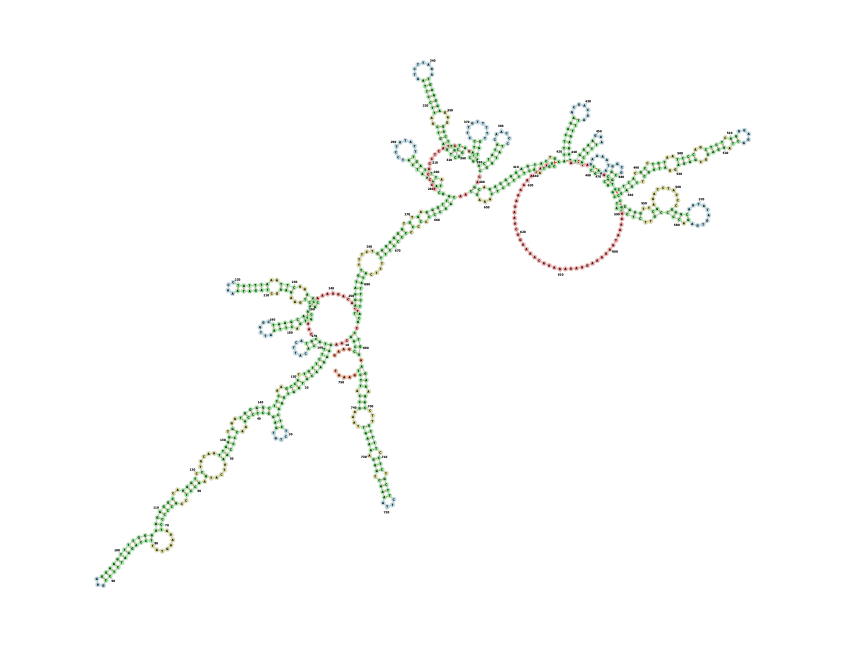
\includegraphics[width=\textwidth]{figs/rnagorilla.png}
    \caption{BC200 RNA Secondary Structure in Gorilla gorilla}
    \label{fig:gorilla-structure}
  \end{subfigure}
  \hfill
  \begin{subfigure}[b]{0.4\textwidth}  
    \centering
    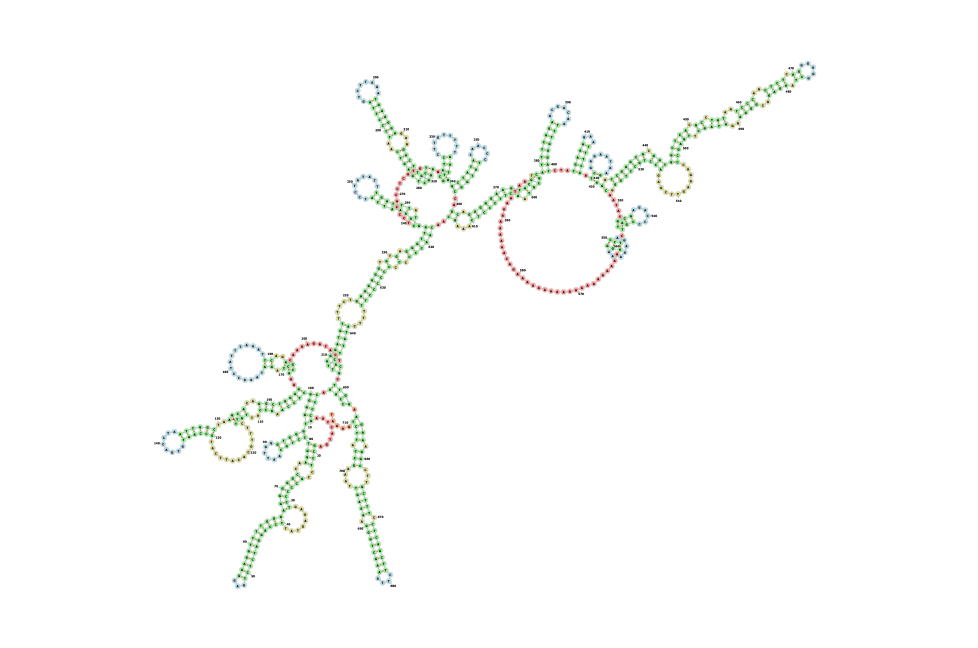
\includegraphics[width=\textwidth]{figs/rnapan.png}
    \caption{BC200 RNA Secondary Structure in Pan paniscus}
    \label{fig:pan-structure}
  \end{subfigure}
  \vskip\baselineskip
  \begin{subfigure}[b]{0.4\textwidth}   
    \centering
    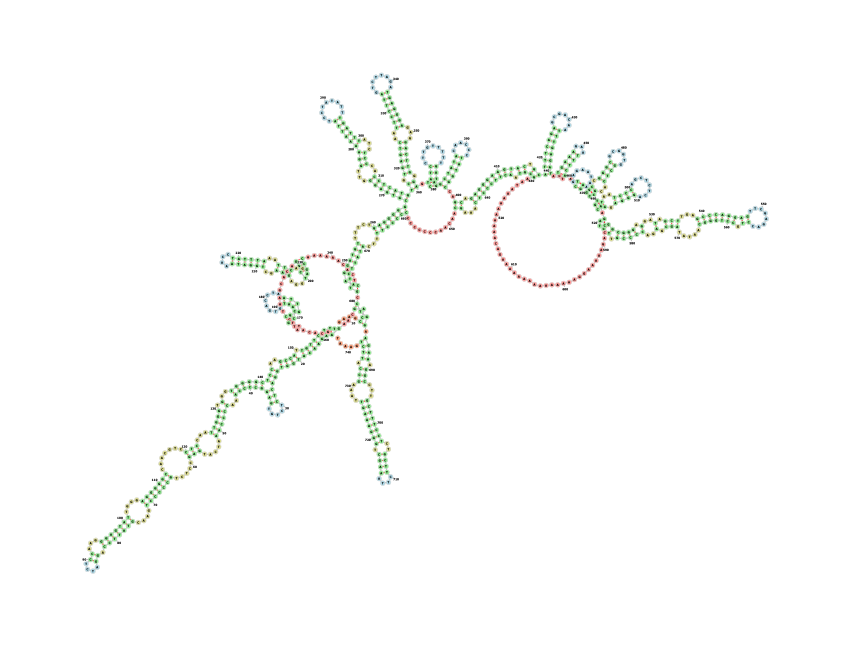
\includegraphics[width=\textwidth]{figs/rnapongo.png}
    \caption{BC200 RNA Secondary Structure in pongo pygmaeus}
    \label{fig:pongo-structure}
  \end{subfigure}
  \hfill
  \begin{subfigure}[b]{0.4\textwidth}   
    \centering
    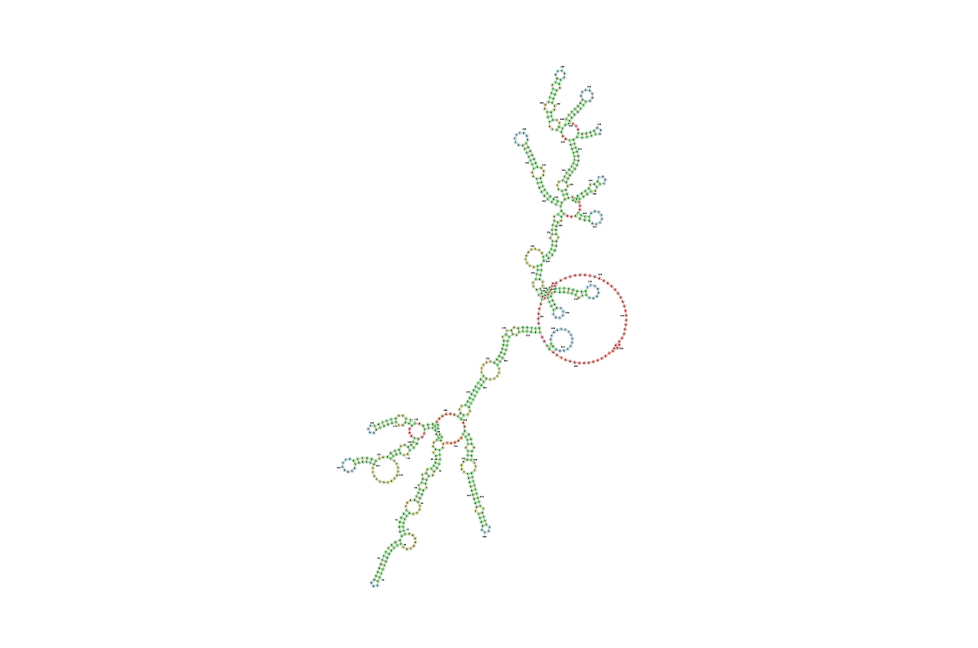
\includegraphics[width=\textwidth]{figs/rnahylobates.png}
    \caption{BC200 RNA Secondary Structure in Hylobates lar}
    \label{fig:hylobates-structure}
  \end{subfigure}
  \caption{RNA Secondary Structures of Hominoidea BC200 Homologs, generated by FORNA \cite{kerpedjiev2015forna} using default parameters}
  \label{fig:rna-sec-structure}
\end{figure*}

\subsection{Finding Conserved Parts of the Sequence}

Using multiple sequence alignment we aligned BC200 with its four mostly related homologs to find the conserved parts of the sequence.
Here is the alignment result:

%\begin{figure}[h]
%  \centering
%  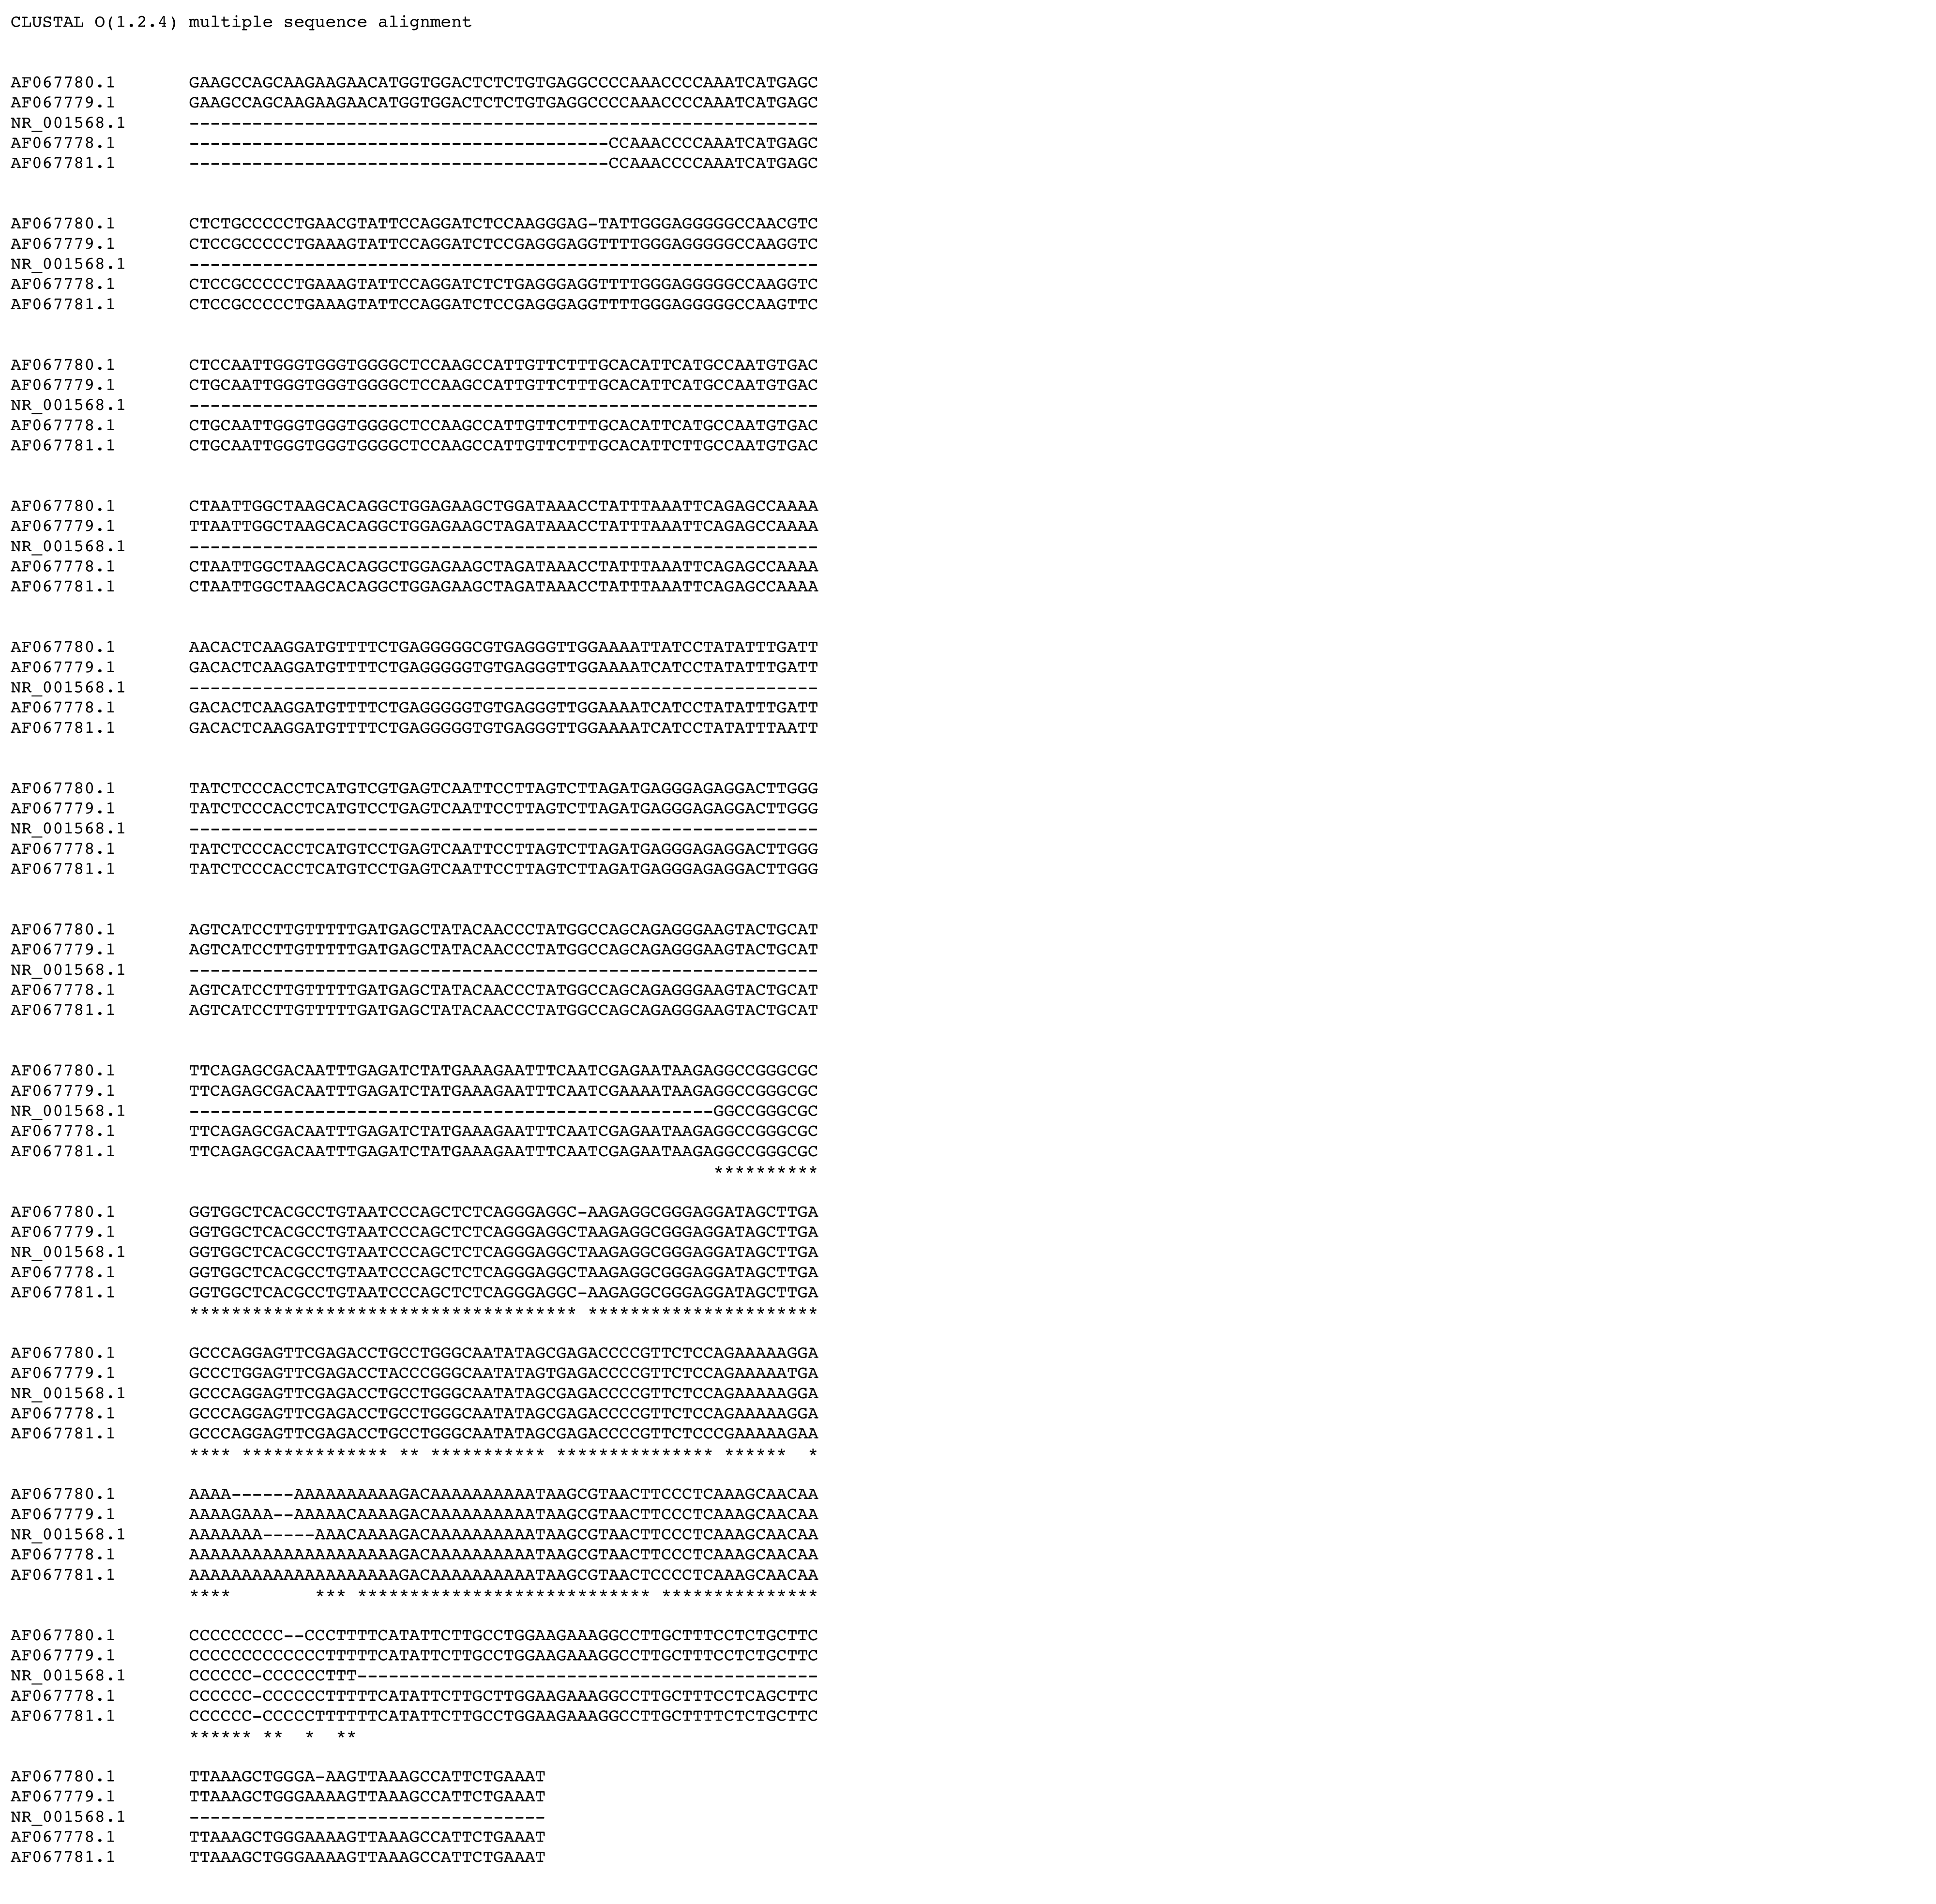
\includegraphics[width=0.4\textwidth]{figs/alignment.png}
%  \caption{BC200 and it's homologs ClustalW alignment Result}
%  \label{fig:alignment result}
%\end{figure}

It can be concluded from the results, most parts of the BC200 sequence are conserved. 
Non-coding sequences important for gene regulation, such as the binding or recognition sites of ribosomes and transcription factors. 
However, sequence conservation in non-coding RNAs is generally poor compared to protein-coding sequences, and base pairs that contribute to structure or function are often conserved instead \cite{johnsson2014evolutionary}. 
So, the result shows that there should be a high similarity between BC200 RNA function in human body and in other species. 
So, the following result does not support our hypothesis, and they suggest that Alzheimer’s can be shared between human and great apes.

\section{Discussion}\label{sec:discussion}
TODO

\section{Conclusion}\label{sec:conclusion}
TODO

\bibliographystyle{IEEEtran}
\bibliography{refs.bib}
\end{document}
